% !TEX root = ./Vorlesungsmitschrift DIFF 2.tex  
\lecture{Mo 15.06. 10:15}{}
Letztes Mal: Legendre, Hermite und Laguerre DGL'n. Lösungen waren explizite Funktionen (Polynome, \( \Ln; \), \dots). Das nicht immer so:
\minisec{Besselsche DGL:} \( \varv\in \reals \).
\begin{equation*}
  y''+\frac{1}{x}y'+\parens*{1-\frac{\varv^2}{x^2}}y=0\quad \text{auf }\reals_{>0}.
\end{equation*}
Lösungen heißen \emph{Zylinder-Funktionen} der Ordnung \( \varv \). Wir machen folgenden Ansatz (absolute Konvergenz voraussetzend)
\begin{equation*}
  u(x)=x^{\rho}\sum_{k=0}^{\infty}a_k x^k.
\end{equation*}
Dann ist
\begin{align*}
  u'(x)&=\rho x^{\rho-1}\sum_{k=0}^{\infty}a_k x^k+x^{\rho-1}\sum_{k=0}^{\infty}x k a_k x^{k-1}\\
  &=x^{\rho-1}\sum_{k=0}^{\infty}(k+\rho)a_k x^k\\
  u''(x)&=x^{\rho-2}\sum_{k=0}^{\infty}(k+\rho)(k+\rho-1)a_k x^k.
\end{align*}
Einsetzen (und mal \( x^{-\rho+2} \) nehmen) liefert für \( x^m \) (unter Verwendung von \( 1-\frac{\varv^2}{x^2}=\frac{x^2-\varv^2}{x^2} \))
\begin{gather*}
  (\rho+m-1)(\rho+m)a_m+(\rho+m)a_m+a_m(-\varv^2)+a_{m-2}=0\\
  a_m((\rho+m)^2-\varv^2)+a_{m-2}=0.
\end{gather*}
Rekursion! \\
\( a_0(\rho^2-\varv^2)=0 \). Wähle \( \rho=\varv \), und setze \( a_0=1 \). \\
\( a_1=(2\varv+1)=0 \). Setze \( a_1=0 \).\\
Es muss gelten
\begin{equation*}
  a_m(2\varv m+m^2)+a_{m-2}=0.
\end{equation*}

Sei \( m=2n+1 \), dann ist \( a_m=0 \), denn \( a_1=0 \) und
\begin{equation*}
  a_{2n+1}(\braceannotate{\text{Ist \( \varv\in\wholes \): gerade}{2\varv(2n+1)}}{\braceannotate{\text{ungerade}}{(2n+1)^2}})\needed{=}0.
\end{equation*}
Wähle also \( a_{2n+1}=0 \).

Ist \( m=2n \), so ist (per Induktion beweisen!) (\( \Gamma \) ist die Gammafunktion).
\begin{equation*}
  a_{2n}=\frac{(-1)^n}{4^n\factorial{n}\braceannotate{=\frac{\Gamma(v+n+1)}{\Gamma(v+1)}}{(\varv+n)\dotsm (v+1)}}
\end{equation*}
\timplies Lösung:
\begin{equation*}
  \besselfirstkind{\varv}{x}=\parens*{\frac{x}{2}}^{\varv}\sum_{n=0}^{\infty}\frac{(-1)^n}{\factorial{n}\Gamma(v+n+1)}\parens*{\frac{x}{2}}^{2n}
\end{equation*}
\enquote{Besselfunktion \ordinalnum{1} Art der Ordnung \( \varv \)}.

Reihe konvergiert absolut, unsere Manipulationen sind also a posteriori gerechtfertigt!

Ist \( \varv\not\in \wholes \), so bilden \( \besselfirstkind;{\varv} \) und \( \besselfirstkind;{v} \) ein Fundamentalsystem. Ist \( \gamma\in \wholes \), kann man \zb die Besselfunktion \ordinalnum{2} Art hinzuziehen, die wir hier aber nicht betrachten.
\begin{figure}[H]
  \centering
  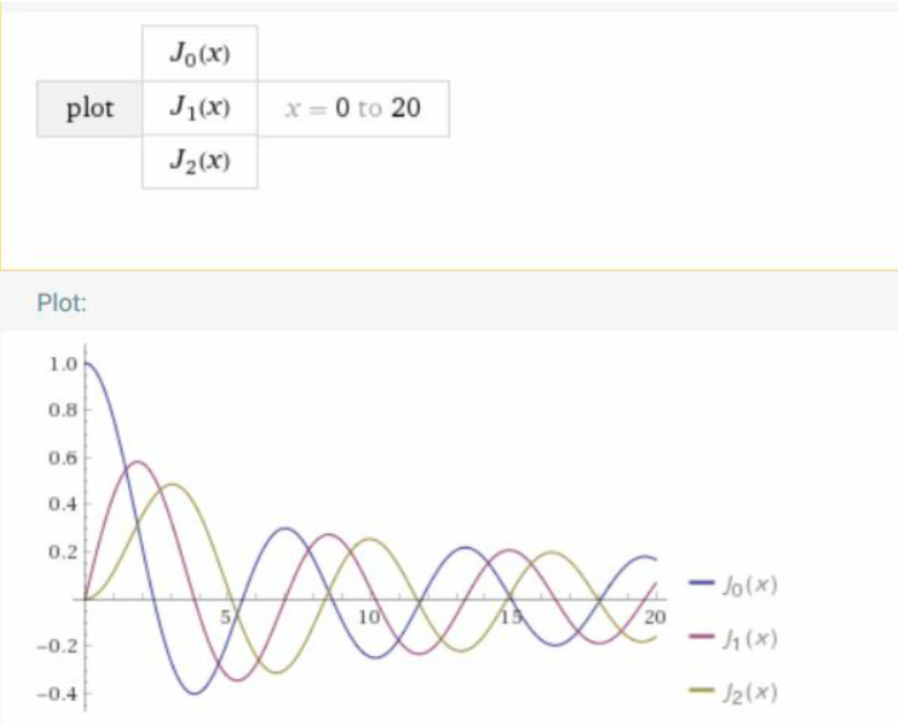
\includegraphics[width=0.5\linewidth]{bessel_funktionen}
  \label{fig:bessel_funktionen}
\end{figure}
Zum Abschluss:
\section{Lineare DGL-Systeme mit konstanten Koeffizienten}
\begin{lemma}\label{eigenwert_von_konstanter_matrix_dgl_liefert_exp_loesung}
  Sei \( A\in \sqmatrices{n}{\complexs} \) und sei \( v\in \complexs^n \) ein Eigenvektor von \( A \) zum Eigenwert \( \lambda\in \complexs \). Dann ist
  \begin{equation*}
    u\maps \reals\to \complexs^n\quad u(t)=ve^{\lambda t}
  \end{equation*}
  eine Lösung von \( x'=Ax \).
\end{lemma}
\begin{proof}
  \begin{equation*}
    u'(t)=v\lambda e^{\lambda t}=\lambda v e^{\lambda t}=A v e^{\lambda t}.
  \end{equation*}
  
\end{proof}
\begin{folgerung*}
  Ist die Matrix \( A \) diagonalisierbar, besitzt also \( \complexs^n \) eine Basis aus Eigenvektoren \( v_1,\dotsc,v_n \) von \( A \), so bilden die Funktionen \( \set{v_1 e^{\lambda_1 t},\dotsc, v_n e^{\lambda_n t}} \) ein Fundamentalsystem (wobei \( Av_j=\lambda_j v_j \logicspace j=1,\dotsc,n\)). Lineare Unabhängigkeit: \( u_j(0)=v_j \) sind linear unabhängig.
\end{folgerung*}
\begin{beispiel*}
  \( A=\begin{pNiceMatrix} 0 & -\alpha \\ \alpha & 0 \end{pNiceMatrix} \) \timplies \( \lambda=\pm i\alpha \). Fundamentalsystem \( \Set{\begin{pNiceMatrix} 1 \\ -i \end{pNiceMatrix}e^{i\alpha t},\begin{pNiceMatrix} 1 \\ i \end{pNiceMatrix}e^{-i\alpha t }} \).
\end{beispiel*}
\begin{bemerkung}
  Ist \( A\in \sqmatrices{n}{\reals} \), so ist mit \( \lambda\in \complexs \) Eigenwert auch \( \conjugate{\lambda} \) Eigenwert und es gilt 
  \begin{equation*}
    Av=\lambda v\iff A\conjugate{v}=\conjugate{\lambda}\conjugate{v}.
  \end{equation*}
  Für \( \lambda\in \complexs\setminus \reals \). Man kann in diesem Fall also immer ein \emph{reelles} Fundamentalsystem finden (\( v+\conjugate{v},v-\conjugate{v}\in  \reals^n \)).
\end{bemerkung}
\begin{beispiel*}
  Gekoppelte Pendel
  \begin{align*}
    mx''=-\frac{mg}{h}x-k(x-y)\\
    my''=-\frac{mg}{y}y-k(y-x)\quad k,m,g,h>0
  \end{align*}
  \begin{figure}[H]
    \centering
    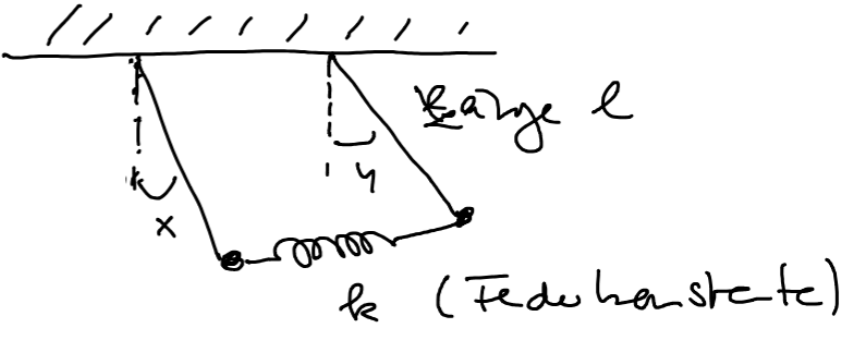
\includegraphics[width=0.5\linewidth]{gekoppeltes_pendel}
    \label{fig:gekoppeltes_pendel}
  \end{figure}
  Reduktion der Ordnung:
  \begin{equation*}
    \begin{pNiceMatrix} x \\ y \\ p \\ q \end{pNiceMatrix}'=\begin{pNiceMatrix} 0 & 0 & 1 & 0 \\ 0 & 0 & 0 & 1 \\ -(w_0^2+k_0) & k_0 & 0 & 0 \\ k_0 & -(w_0^2+k_0) & 0 & 0 \end{pNiceMatrix}\begin{pNiceMatrix} x \\ y \\ p \\ q \end{pNiceMatrix}.
  \end{equation*}
  \( w_0=\sqrt{\frac{g}{l}} \), \( k_0=\frac{k}{m} \). Eigenwerte \( \pm iw_0 \), \( \pm i\sqrt{w_0^2+2k_0}\defines \pm iw \). Eigenvektoren
  \begin{equation*}
    v_1=\begin{pNiceMatrix} 1 \\ 1 \\ iw_0 \\ iw_0 \end{pNiceMatrix}\quad \bar{v}_1=\begin{pNiceMatrix} 1 \\ 1 \\ -iw_0\\ iw_0 \end{pNiceMatrix}\quad v_2=\begin{pNiceMatrix} 1 \\ -1 \\ iw \\ -iw \end{pNiceMatrix}\quad \bar{v}_2=\begin{pNiceMatrix} 1 \\ -1 \\ -iw \\ iw \end{pNiceMatrix}.
  \end{equation*}
  Reelles Fundamentalsystem
  \begin{gather*}
    e^{+iw_0t}v_1+e^{-iw_0 t} \bar{v}_1\\
    -i\p*{e^{+iw_0t}v_1-e^{-iw_0 t} \bar{v}_1}\\
    e^{+iwt}v_1+e^{-iw t} \bar{v}_1\\
    -i\p*{e^{+iwt}v_1-e^{-iw t} \bar{v}_1}.
  \end{gather*}
\end{beispiel*}
\begin{spezialfall}\label{diagonalisierbare_lineare_dgl_spezialfall}
  Sei \( A \) diagonalisierbar. Entstehe \( A \) aus DGL \( n \)-ter Ordnung: \( x^{(n)}+a_{n-1}x^{(n-1)}+\dotsb+ a_1x'+a_0 x=0 \)
  \begin{equation*}
    \begin{pNiceMatrix} x_0 \\ x_1 \\ \Vdots \\ x_{n-2} \\ x_{n-1} \end{pNiceMatrix}'=\braceannotate{=A\in \sqmatrices{n}{\mathbb{K}}}{\begin{pNiceMatrix} 0 & 1 \\  & 0 & 1 \\  &  &  \Ddots & \Ddots \\\\ & & & & 0 & 1 \\ -a_0 & -a_1 & -a_2 & \Cdots & -a_{n-2} & -a_{n-1} \end{pNiceMatrix}}\begin{pNiceMatrix} x_0 \\ x_1 \\ \Vdots \\ x_{n-2} \\ x_{n-1} \end{pNiceMatrix}
  \end{equation*}
  Dann ist \( \set{x_j e^{\lambda_j t}|v_j=1,\dotsc, n} \) it \( (v_1,\dotsc,v_n) \) Basis von \( \mathbb{K}^n \) und \( A v_j=\lambda_j v_j \) ein Fundamentalsystem. Die Null-Komponenten \( v_{j,0}e^{\lambda_j t} \) sind dann zwar Lösungen der DGL \( n \)-ter Ordnung, aber nicht unbedingt linear unabhängig: zwar ist \( v_{j,0}\neq 0 \) (sonst wäre \( v_j=0 \)), aber wenn ein Eigenwert mit höherer Multiplizität als \( 1 \) vorkommt, wären die Funktionen linear abhängig.
\end{spezialfall}
Es gilt jedoch:
\begin{folgerung}
  Sei eine DGL
  \begin{equation}
    \parendiff{x}{n}+a_{n-1}\parendiff{x}{n-1}+\dotsb+a_1 x'+a_0 x=0
  \end{equation}
  \( a_j \in \complexs \), gegeben. Das Polynom
  \begin{equation*}
    T^n+a_{n-1}T^{n-1}+\dotsb+a_1 T+a_0=0
  \end{equation*}
  habe \( n \) paarweise verschiedene Nullstellen \( \lambda_1,\dotsc,\lambda_n \in \complexs\). Dann ist \( \Phi=(e^{\lambda_1 t},\dotsc,e^{\lambda_n t}) \) ein Fundamentalsystem für die DGL\@.
\end{folgerung}
\begin{proof}
  Das charakteristische Polynom der gegebenen Matrix ist
  \begin{equation*}
    \lambda_n + a_{n-1}\lambda^{n-1}+\dotsb+a_1 \lambda+a_0.
  \end{equation*}
\end{proof}
\begin{beispiel*}
  \( \parendiff{x}{4}-6\parendiff{x}{3}+11\parendiff{x}{2}-6x=0 \).
  \begin{equation*}
    T^4-6T^3+11T^2-6T=T(T-1)(T-2)(T-3)
  \end{equation*}
  \timplies \( (1,e^t,e^{2t},e^{3t}) \) ist ein Fundamentalsystem.

  Mehrfache Nullstellen \tto allgemeiner in Zusammenhang mit triangulierbaren Matrizen.
\end{beispiel*}
\begin{lemma}
  Sei \( A\in \sqmatrices{n}{C} \), \( S\in \invertiblematrices{n}{\complexs} \). Dann gilt: \( u\maps \reals\to \complexs^n \) ist genau dann Lösung der DGL \( x'=Ax \), wenn \( \tilde{u}\definedas \inverse{S}u \maps \reals\to \complexs^n \) Lösung von \( y'\definedas \braceannotate{B}{\inverse{S}AS}y \).
\end{lemma}
\begin{proof}
  \begin{gather*}
    u'(t)=A u(t)\\
    \iff \equalto{(\inverse{S}u)'(t)}{\inverse{S}\matrixmult u'(t)}=\inverse{S}\matrixmult A u(t)=(\inverse{S}A S)\inverse{S}u(t).
  \end{gather*}  
\end{proof}
\begin{bemerkung*}
  Sei \( A\in \sqmatrices{n}{\complexs} \). Dann gibt es \( S\in \invertiblematrices{n}{\complexs} \), \sd \( \inverse{S}AS \) Jordan-Form besitzt, also von der Form
  \begin{figure}[H]
    \centering
    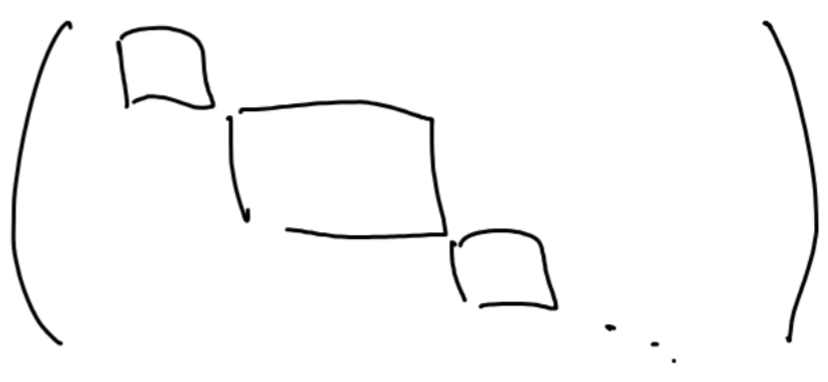
\includegraphics[width=0.3\linewidth]{jordanform}
    \label{fig:jordanform}
  \end{figure}
  ist, wobei jedes Kästchen 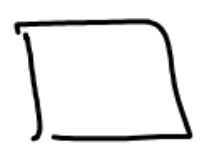
\includegraphics[height=\baselineskip]{kaestchen} von der Form
  \begin{figure}[H]
    \centering
    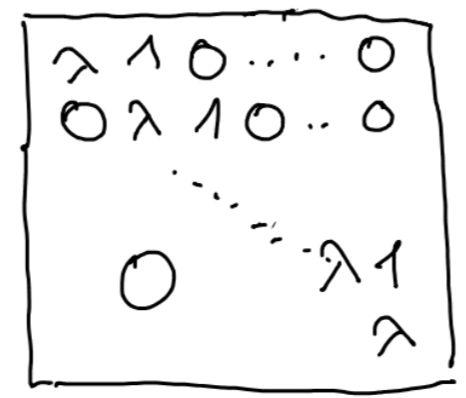
\includegraphics[width=0.3\linewidth]{kaestchenform}
    \label{fig:kaestchenform}
  \end{figure}
  ist.
\end{bemerkung*}
\begin{satz}\label{jordanform_liefert_lineare_dgl_loesung}
  Sei \( A\in \sqmatrices{n}{\complexs} \). Sei \( B=\inverse{S}A S \) die Jordan-Form von \(  A\). Seien \( J_1,\dots, J_k \) die Jordan-Kästchen von \( B \) zum Eigenwert \( \lambda_1,\dots,\lambda_k \) und seien sie der Größe \( n_1\times n_1,\dotsc, n_k \times n_k \). Dann bildet
  \begin{align*}
    e^{\lambda_1 t}\begin{pNiceMatrix} 1 \\ 0 \\ \Vdots \\ \\ 0 \end{pNiceMatrix}, &&e^{\lambda_1 t}\begin{pNiceMatrix} \frac{t}{\factorial{1}} \\ 1 \\ \Vdots \\ \\ 0 \end{pNiceMatrix},&&e^{\lambda_1}\begin{pNiceMatrix} \frac{t^2}{\factorial{2}} \\ \frac{t}{\factorial{1}} \\ 1 \\ \Vdots \\ 0 \end{pNiceMatrix}, &&\dotsc, &&e^{\lambda_1 t} \begin{pNiceMatrix} \frac{t^{n_1-1}}{\factorial+{n_1-1} }\\ \Vdots \\ t \\1\\ 0 \\ \Vdots \\ 0 \end{pNiceMatrix},\\
    e^{\lambda_2 t}\begin{pNiceMatrix} 0 \\ \Vdots_{n_1} \\ 0 \\ 1\\ 0\\ \Vdots \\  \hphantom{0}1\hphantom{0}\  \end{pNiceMatrix},&&e^{\lambda_2 t}\begin{pNiceMatrix} 0 \\ \Vdots_{n_1} \\ 0 \\ t\\  \hphantom{0}1\hphantom{0} \\ \Vdots \\ 0  \end{pNiceMatrix},&&\dotsc\\
    \dotsc && && && \dotsc, &&e^{\lambda_k}\begin{pNiceMatrix} 0 \\ \Vdots \\ 0 \\ \frac{t^{n_k-1}}{\factorial{n_{k}-1}} \\ \Vdots_{n_k} \\ t \\ 1 \end{pNiceMatrix}
  \end{align*}
  ein Fundamentalsystem \( \tilde{\Phi} \) von \( y'=By \) und somit ist \( \Phi=S\tilde{\Phi} \) ein Fundamentalsystem von \( x'=Ax \).
\end{satz}
\timestamp{18:00}
\begin{proof}
  Für ein Jordan-Kästchen \( J \) von \( B \). Wir betrachten also \( z'=Jz \),
  \begin{align*}
    J&=\begin{pNiceMatrix}
      \lambda & 1 &  \\
       & \lambda & 1 \\
       &  & \Ddots & \Ddots \\
       & & & & 1\\
       & & & & \lambda
    \end{pNiceMatrix}\quad m\times m\\
    z_1'&=\lambda z_1+z_2\\
    z_2'&=\lambda z_2+z_3\\
    &\vdots \\
    z_{m-1}'&=\lambda z_{m-1}+z_m\\
    z_m'&=\lambda z_m\\
    \implies v_m(t)&=e^{\lambda t}\\
    \implies z_{m-1}'-\lambda z_{m-1}&=e^{\lambda t} 
  \end{align*}
  Mit \ref{variation_der_konstanten_die_zweite} lösen.
  \begin{align*}
    v_{n-1}(t)&=e^{\lambda t}\Integrate{\frac{1}{e^{\lambda t}} e^{\lambda t}}{t}=e^{\lambda t}\cdot t\\
    \implies z_{m-2}'-\lambda z_{m-2}&= te^{\lambda t}.
  \end{align*}
  Mit \ref{variation_der_konstanten_die_zweite}:
  \begin{equation*}
    v_{m-2}(t)=e^{\lambda t}\Integrate{t}{t}=e^{\lambda t}\frac{t^2}{2}
  \end{equation*}
  \timplies \Beh (per Induktion):
  \begin{equation*}
    v_{m-k}(t)=e^{\lambda t}\Integrate{\frac{t^{k-1}}{\factorial+{k-1}}}{t}=e^{\lambda t}\frac{t^k}{\factorial{k}},
  \end{equation*}
  denn die lineare Unabhängigkeit ist offensichtlich, und \( S\tilde{\Phi} \) ist auch linear unabhängig (\( S\in \invertiblematrices{n}{\complexs} \)).
  
\end{proof}
\begin{bemerkung*}
  Insbesondere folgt \thref{eigenwert_von_konstanter_matrix_dgl_liefert_exp_loesung} und \ref{diagonalisierbare_lineare_dgl_spezialfall}:\\
  Ist \( B=\inverse{S}AS \) diagonal, so ist \( \set{e^{\lambda j} e_j|j=1,\dotsc, n} \) Fundamentalsystem und \( S e_j= \) \( j \)-te Spalte von S \( = \) Eigenvektor zu \( \lambda_j \).

  Die Jordanzerlegung zu berechnen, ist aufwendig (für große \( n \)). Liegt eine obere Dreiecks-Matrix vor, kann man auch vorgehen wie folgt:
\end{bemerkung*}
\begin{bemerkung}
  Habe \( B\in \sqmatrices{n}{\complexs} \) obere Dreiecksgestalt. Betrachte die DGL \( y'=By \) also
  \begin{align*}
    y_1'&=&&B_{11}y_1&&+&&B_{12}y_2&&+&&\dotsb&&+&&B_{1,n-1}y_{n-1}&&+&&B_{1,n}y_n\\
    y_2'&=&&&&&&B_{22}y_2&&+&&\dotsb&&+&&B_{2,n-1}y_{n-1}&&+&&B_{2,n}y_n\\
    &\vdots\\
    y_{n-1}'&=&&&&&&&&&&&&&&B_{n-1,n-1}y_{n-1}&&+&&B_{n-1,n}y_n\\
    y_n'&=&&&&&&&&&&&&&&&&&&B_{n,n}y_n.
  \end{align*}
  mit Anfangsbedingung
  \begin{equation*}
    y(t_0)=y_0=\begin{pNiceMatrix} y_{0,1} \\ \Vdots \\ y_{0,n} \end{pNiceMatrix}.
  \end{equation*}
  Dann erhält man sukzessive eine Lösung \( v\maps \reals\to \complexs^n \) von \( y'=By \):
  \begin{enumerate}[label=\rechtsklammer{\arabic*}]
    \item \( y_n'=B_{nn}y_n \) \timplies \( v_n(t)=C_n e^{B_{nn}t} \) (\( C_n e^{B_{nn}t_0}=y_{0n} \))
    \item \( y_{n-1}'-B_{n-1,n-1}y_{n-1}=B_{n-1,n}C_n e^{B_{nn}t} \) inhomogene Gleichung. Mit \thref{variation_der_konstanten_die_zweite} bestimme ein Fundamentalsystem und eine spezielle Lösung. Passe wieder die Konstanten an\dots
    \item[\rechtsklammer{k}] \( v_n, v_{n-1},\dotsc, v_{k+1} \) sind schon bestimmt. FÜr \( v_k \) ergibt sich
    \begin{equation*}
      y_k'-B_{kk}y_k=\sum_{j=k+1}^{n}B_{kj}v_j(t)
    \end{equation*}
    \usf.\timestamp{23:10}
  \end{enumerate}
  Auch Gleichungen wie in \ref{diagonalisierbare_lineare_dgl_spezialfall}, die mit Reduktion der Ordnung aus einer Gleichung \( n \)-ter Ordnung hervorgingen, lassen sich durch den Umweg über die Jordan-Form (\ref{jordanform_liefert_lineare_dgl_loesung}) lösen. Wir gehen direkter vor:
\end{bemerkung}
\begin{lemma}\label{fundamentalsystem_homogene_lineare_dgl_nter_ordnungW}
  Betrachte \( \parendiff{n}{x}+a_{n-1}\parendiff{x}{n-1}+\dotsb+a_0 x=0  \). Es gelte
  \begin{equation*}
    p(T)\definedas T^n+ a_{n-1}T^{n-1}+\dotsb+a_1 T+a_0=(T-\lambda_1)^{k_1}\dotsm (T-\lambda_r)^{k_r}
  \end{equation*}
  mit \( \lambda_j \) paarweise verschieden, so bildet
  \begin{equation*}
    u_{j,i}(t)=t^i e^{\lambda_j t}\quad i\in \set{0,\dotsc,k_j -1}\logicspace j\in \set{1,\dotsc,r}
  \end{equation*}
  ein Fundamentalsystem.
\end{lemma}
\begin{proof}
  \( u_{j,i}(t) \) ist Lösung:
  \begin{equation*}
    (T-\lambda_1)^{k_1}\dotsm (T-\lambda_r)^{k_r}=\prod_{s\neq j}(T-\lambda_s)^{k_s}\cdot(T-\lambda_j)^{k_j}.
  \end{equation*}
  Setze \( \odv{}{t} \) für \( T \) ein und wende den Ausdruck auf \( u_{j,i} \) an. \Dh, wir prüfen, ob \( u_{j,i} \) die DGL erfüllt. Zunächst eine Hilfs-Aussage: Es gilt
  \begin{equation*}
    \p*{\odv{}{t}-\lambda}^k \p*{f(t)e^{\lambda t}}=\parendiff{f}{k}(t)e^{\lambda t}\quad f\in \stetigefunktionen[k]
  \end{equation*}
  \begin{subproof}[per Induktion]
    \begin{proofdescription}
      \item[\( k=0 \)] \checkmark
      \item[\( k \to k+1 \)] \begin{equation*}
        \p*{\odv{}{t}-\lambda}\p*{\odv{}{t}-\lambda}^k\p{f(t)e^{\lambda t}}=\p*{\odv{}{t}-\lambda}\p*{\parendiff{f}{k}(t)e^{\lambda t}}=\parendiff{f}{k+1}(t)e^{\lambda t}+\parendiff{f}{k}(t)\p*{\lambda e^{\lambda t}-\lambda e^{\lambda t}}.
      \end{equation*} 
    \end{proofdescription}
  \end{subproof}
  Also ist
  \begin{align*}
    p\p*{\odv{}{t}} u_{j,i}(t)&=\prod_{j\neq j} \p*{\odv{}{t}-\lambda_k}^{k_l}\cdot \p*{\odv{}{t}-\lambda_j}^{k_j}\p*{t^i e^{\lambda_j t}}\\
    &=\prod_{j\neq j}\p*{\odv{}{t}-\lambda_l}^{k_l}\braceannotate{=0 \text{, da \( i<k_j \)}}{\odv[k_j]{(t^i)}{t}}\cdot e^{\lambda_j t}.
  \end{align*}
  Lineare Unabhängigkeit
  \begin{equation*}
    \wronskideterminant{0}=\determinant+*{\begin{pNiceMatrix}[first-row,first-col]
       &  &   &   & k_1 \text{-te} &  & & (k_1+k_2)\text{-te}     \\
       & 1 & 0 & \Cdots & 0 & 1 & \Cdots & 0 & \Cdots &  \\
       & \lambda_1 & 1 &  & \Vdots & \lambda_2 &  & \Vdots &  &  \\
       & \Vdots & \lambda_1 &  &  & \Vdots  &  &  &  &  \\
       \\
       k_1 \text{-te}&  & \Vdots &  & 1 &   &  &  &  &  \\
       &  &  &  & \lambda_1 &   &  &  &  &  \\
       \\
       k_2 \text{-te} &  &  &  & \Vdots &   &  & 1 &  &  \\
        &  &  &  & \Vdots &   &  & \Vdots &  &  \\
       & \lambda_1^{n-1} & \lambda_1^{n-2}&\Cdots & \lambda_1^{n-k_1} &\lambda_2^{n-1}&\Cdots& \lambda_1^{n-k_2} & \Cdots 
    \end{pNiceMatrix}},
  \end{equation*}
  denn
  \begin{equation*}
    \braceannotate{\sum_{r=0}^{l}\parendiff+{t^i}{r}\lambda^r e^{\lambda t}}{\odv[l]{\p*{t^i e^{\lambda t}}}{t}_{t=0}}=
    \begin{cases}
      0 & l<i\\
      1 & l=i\\
      \lambda^{l-i}& l>i.
    \end{cases}
  \end{equation*}
  Also
  \begin{equation*}
    W(0)=\determinant-{\raisebox{-2\baselineskip}{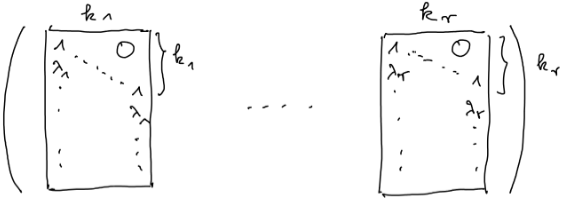
\includegraphics[height=5\baselineskip]{wronski_determinante_fundamentalsystem_n_te_lineare_dgl}}}. % ChkTeX 25
  \end{equation*}
  Da die \( \lambda_j \) paarweise verschieden sind, sind die Spalten linear unabhängig \timplies \( W(0)\neq 0 \).
\end{proof}
\begin{beispiel*}
  \begin{gather*}
    \parendiff{x}{4}+8\parendiff{x}{2}+1=0\\
    T^4+8T^2+16 \begin{aligned}[t]
      &=(T^2+4)^2\\
      &=(T-2i)^2(T+2i)^2
    \end{aligned}\\
    \lambda_1=2_i\quad \lambda_2=-2_i\\
    \begin{aligned}[t]
      u_{1,0}(t)&=e^{2_i t}, & u_{2,0}(t)&=e^{-2it}\\
      u_{1,1}(t)&=te^{2_i t}, & u_{2,1}(t)&=te^{-2it}.
    \end{aligned}
  \end{gather*}
\end{beispiel*}
\timestamp{34:05}
\begin{bemerkung*}
  Inhomogene Gleichungen löst man über das zugehörige System \ordinalnum{1} Ordnung und Variation der Konstanten. In speziellen Fällen kann man auch anders vorgehen:
\end{bemerkung*}
\begin{lemma}
  Sei \( b(t)=f(t)e^{\alpha t} \) mit \( \alpha= \) Nullstelle \( k \)-ter Ordnung (\( k\geq 0 \)) des Polynoms
  \begin{equation*}
    p(T)=T^n+a_{n-1} T^{n-1}+\dotsb+a_1 T+a_0
  \end{equation*}
  und wo \( f \) ein Polynom der Ordnung \( m \) ist. Dann besitzt die DGL
  \begin{equation*}
    p \p*{\odv{}{t}}x=b(t)
  \end{equation*}
  eine spezielle Lösung \( v\maps \reals\to \complexs \) der Gestalt
  \begin{equation*}
    v(t)=h(t) e^{\alpha t},
  \end{equation*}
  wobei \( h \) ein Polynom von Grad \( m+k \) ist.
\end{lemma}
\begin{proof}
  \( p(t)=q(T)(T-\alpha)^k \), \( q(\alpha)\neq 0  \).
  Induktion:
  \begin{proofdescription}
    \item[\( m=0 \)]
    \begin{equation*}
      p\p*{\odv{}{t}}x= ce^{\alpha t}
    \end{equation*}
    \begin{behauptung*}
      \( v(t)=\frac{c}{\factorial{k}q(a)}t^k e^{\alpha t} \) ist Lösung.
    \end{behauptung*}
    \begin{subproof}
      \begin{align*}
        p\p*{\odv{}{t}}v&=\frac{c}{\factorial{k}q(a)}q\p*{\odv{}{t}}\cdot \explain{\text{wie im Beweis von \ref{fundamentalsystem_homogene_lineare_dgl_nter_ordnungW}}}{\parendiff+*{t^k}{k}}\matrixmult e^{\alpha t}\\
        &=\frac{c}{\factorial{k}q(\alpha)}e^{\alpha t}\\
        &=\frac{c}{\factorial{k}q(\alpha)}\factorial{k} q(\alpha)e^{\alpha t}.
      \end{align*}
    \end{subproof}
    \item[\( m-1\to m \)] Es gilt
    \begin{align*}
      p\p*{\odv{}{t}}\p*{t^{m+k}e^{\alpha t}}&=q\p*{\odv{}{t}}\p*{\odv{}{t}-\alpha}^k\p*{t^{m+k}e^{\alpha t}}\\
      &=q\p*{\odv{}{t}}\p*{\frac{\factorial+{m+k}}{\factorial{m}}t^m e^{\alpha t}}=\braceannotate{\mathclap{\text{Polynom von Grad \( m \)}}}{g(t)}e^{\alpha t}.
    \end{align*}
    Für geeignetes \( c\neq 0 \) ist daher \( f_1\definedas f-cg \) ein Polynom von Grad \( m-1 \). Nach Induktionsvoraussetzung gibt es ein Polynom \( h_1 \) von Grad \( m-1+k \) \sd 
    \begin{equation*}
      p\p*{\odv{d}{t}}\p*{h_1(t)e^{\alpha t}}=f_1(t) e^{\alpha t}.
    \end{equation*}
    Dann ist
    \begin{equation*}
      h(t)\definedas h_1(t)+c t^{m+k}
    \end{equation*}
    Polynom von Grad \( m+k \) und es gilt 
    \begin{equation*}
      p\p*{\odv{}{t}}\p*{h(t)e^{\alpha t}}=f_1(t)e^{\alpha t}+\braceannotate{cg(t)e^{\alpha t}}{p\p*{\odv{}{t}}\p*{ct^{m+k}e^{\alpha t}}}.
    \end{equation*}
  \end{proofdescription}
\end{proof}
\begin{beispiel*}
  \( \parendiff{x}{3}+2\parendiff{x}{2}+x'=t+2e^{-t}\). Homogene Gleichung: 
  \begin{equation*}
    p(T)=T^3+2T^2+T=T(T+1)^2.
  \end{equation*}
  \timplies \( \lambda_1=-1 \) (Vielfachheit \( 2 \)), \( \lambda_2=0 \). \timplies Fundamentalsystem \( (e^{-t},te^{-t},1) \). Inhomogene Gleichung: Wir zerlegen die rechte Seite und lösen
  \begin{equation*}
    \tag{1}\label{eq:inhomogene_polynom_dgl_linearer_teil}p\p*{\odv{}{t}}x=t
  \end{equation*}
  und
  \begin{equation*}
    \tag{2}\label{eq:inhomogene_polynom_dgl_exponentieller_teil}p\p*{\odv{}{t}}x=2e^{-t}.
  \end{equation*}
  Addition der Lösungen liefert die gesuchte Lösung:
  \begin{proofdescription}
    \item[\eqref{eq:inhomogene_polynom_dgl_linearer_teil}] Ansatz: \( v_1(t)=C_1 t+C_2 t^2 \) (\( C_0 \) unnötig, da Lösung der homogenen Gleichung) Einsetzen in \eqref{eq:inhomogene_polynom_dgl_linearer_teil} \timplies \( c_1=\frac{1}{2} \), \( c_2=-2 \).
    \item[\eqref{eq:inhomogene_polynom_dgl_exponentieller_teil}] \( v_2(t)=ct^2 e^{-t} \) (\( te^{-t} \) und \( 1 \) sind Lösung der homogenen). Einsetzen in \eqref{eq:inhomogene_polynom_dgl_exponentieller_teil} \timplies \( C=-1 \). Eine spezielle Lösung ist also 
    \begin{equation*}
      v(t)=-2t+\frac{1}{2}t^2-t^2e^{-t}.
    \end{equation*}
  \end{proofdescription}
\end{beispiel*}